\section{Auswertung}
\label{sec:Auswertung}


Die Graphen werden sowohl mit Matplotlib \cite{matplotlib} als auch NumPy \cite{numpy} erstellt. Die Fehlerrechnung wird mithilfe von Uncertainties \cite{uncertainties} 
durchgeführt.
\newline\newline
Der gemessene Dunkelstrom beträgt $I_.{Du}=\SI{3,4e-10}{\metre}$.
Die Wellenlänge des Lasers beträgt $\lambda = \SI{635e-9}{\metre}$, der Abstand zwischen Spalt und Detektor $L=\SI{1}{\metre}$.
\subsection{Beugung am Einzelspalt}

Die Messwerte zur Bestimmung der Spaltbreite $b$ eines Einzelspalts sind in Tabelle \ref{tab:1} zu finden. Dabei wird $I_.{eff}$ über Gleichung \eqref{eq:} berechnet.
Mit einer Regression der Form 
\[
I(\Delta x)=A^2_.0\cdot b^2\cdot\left(
\frac{\lambda}{\pi b \sin{\left(\frac{\Delta x-x_.0}{L}\right)}}\right)^2\cdot\sin^2{\left(\frac{\pi b\sin{\left(\frac{\Delta x-x_.0}{L}\right)}}{\lambda}\right)}
\]
ergibt sich mit den Startwerten
\begin{align*}
p_.0 = (x_.0&=\SI{e-3}{\metre}\text{,}\\
		A_.0&=\SI{10}{\sqrt{\ampere}\per\metre}\text{,}\\
		b	&=\SI{7,5e-5}{\metre})\\
\end{align*}
für die Parameter
\begin{align*}
x_.0&= \SI{2,7(5)e-5}{\metre}\text{,} \\
A_.0&= \SI{5,71(2)}{\sqrt{\ampere}\per\metre}\text{,} \\
b   &= \SI{8,22(3)e-5}{\metre}\text{.} \\
\end{align*}
Der zugehörige Graph ist in Abbildung \ref{fig:Einzel} zu sehen.

\begin{table}
\caption{Messdaten der Stromintensitäten des Interferenzmusters eines Einzelspalts bis zum 1. Nebenmaximum}
\label{tab:tabEinzel}
	\sisetup{table-format=1.2}
	\begin{tabular}{S[table-format=2.2]S[table-format=1.3]S[table-format=1.3]}
		\toprule
		{$\Delta x/10^{-3}\si{\metre}$} & {$I_.{mess}/10^{-7}\si{\ampere}$} & {$I_.{eff}/10^{-7}\si{\ampere}$} \\
		\midrule
		-13.00 & 0.070 & 0.067 \\
		-12.50 & 0.090 & 0.087 \\
		-12.00 & 0.110 & 0.107 \\
		-11.25 & 0.130 & 0.127 \\
		-10.75 & 0.135 & 0.132 \\
		-10.25 & 0.135 & 0.132 \\
		-9.50 & 0.110 & 0.107 \\
		-9.00 & 0.080 & 0.077 \\
		-8.75 & 0.078 & 0.075 \\
		-8.50 & 0.065 & 0.062 \\
		-8.25 & 0.053 & 0.050 \\
		-8.00 & 0.040 & 0.037 \\
		-7.50 & 0.026 & 0.023 \\
		-7.00 & 0.028 & 0.025 \\
		-6.50 & 0.050 & 0.047 \\
		-6.25 & 0.070 & 0.067 \\
		-6.00 & 0.100 & 0.097 \\
		-5.75 & 0.140 & 0.137 \\
		-5.50 & 0.180 & 0.177 \\
		-5.25 & 0.200 & 0.197 \\
		-5.00 & 0.250 & 0.247 \\
		-4.75 & 0.300 & 0.297 \\
		-4.50 & 0.350 & 0.347 \\
		-4.25 & 0.500 & 0.497 \\
		-4.00 & 0.550 & 0.547 \\
		-3.75 & 0.650 & 0.647 \\
		-3.50 & 0.750 & 0.747 \\
		-3.25 & 0.900 & 0.897 \\
		-3.00 & 1.000 & 0.997 \\
		-2.75 & 1.100 & 1.097 \\
		-2.25 & 1.400 & 1.397 \\
		-1.50 & 1.650 & 1.647 \\
		-0.75 & 1.950 & 1.947 \\
		0.00 & 2.250 & 2.247 \\
		\bottomrule
	\end{tabular}

\label{tab:tabEinzel2}
	\sisetup{table-format=1.2}
	\begin{tabular}{S[table-format=2.2]S[table-format=1.3]S[table-format=1.3]}
		\toprule
		{$\Delta x/10^{-3}\si{\metre}$} & {$I_.{mess}/10^{-7}\si{\ampere}$} & {$I_.{eff}/10^{-7}\si{\ampere}$} \\
		\midrule
		0.75 & 2.150 & 2.147 \\
		1.50 & 2.150 & 2.147 \\
		2.25 & 1.900 & 1.897 \\
		2.75 & 1.750 & 1.747 \\
		3.00 & 1.600 & 1.597 \\
		3.25 & 1.500 & 1.497 \\
		3.50 & 1.350 & 1.347 \\
		3.75 & 1.250 & 1.247 \\
		4.00 & 1.100 & 1.097 \\
		4.25 & 1.000 & 0.997 \\
		4.50 & 0.850 & 0.847 \\
		4.75 & 0.750 & 0.747 \\
		5.00 & 0.650 & 0.647 \\
		5.25 & 0.550 & 0.547 \\
		5.50 & 0.500 & 0.497 \\
		5.75 & 0.400 & 0.397 \\
		6.00 & 0.300 & 0.297 \\
		6.25 & 0.250 & 0.247 \\
		6.50 & 0.200 & 0.197 \\
		7.00 & 0.150 & 0.147 \\
		7.50 & 0.075 & 0.072 \\
		8.00 & 0.035 & 0.032 \\
		8.25 & 0.026 & 0.023 \\
		8.50 & 0.019 & 0.016 \\
		8.75 & 0.018 & 0.015 \\
		9.00 & 0.019 & 0.016 \\
		9.50 & 0.032 & 0.029 \\
		10.25 & 0.060 & 0.057 \\
		10.75 & 0.080 & 0.077 \\
		11.25 & 0.094 & 0.091 \\
		12.00 & 0.100 & 0.097 \\
		12.50 & 0.100 & 0.097 \\
		13.00 & 0.090 & 0.087 \\
		\bottomrule
	\end{tabular}

\label{tab:1}
\end{table}

\begin{figure}
\centering
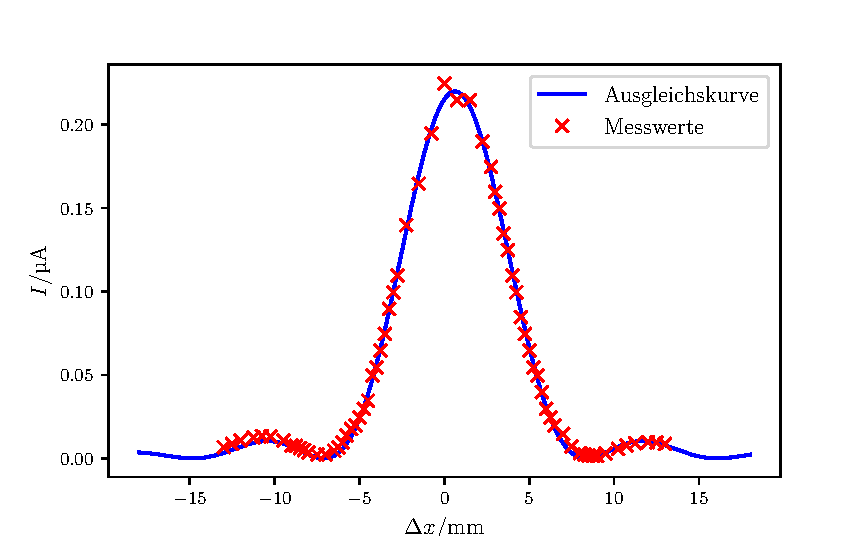
\includegraphics[width=\linewidth-70pt,height=\textheight-70pt,keepaspectratio]{content/images/Einzelspalt.pdf}
\caption{Interferenzmuster der Stromintensitäten eines Einzelspalts in Abhängigkeit von der Verschiebung des Detektors}
\label{fig:Einzel}
\end{figure}

\subsection{Beugung am Doppelspalt}
Die Messwerte zur Bestimmung der Spaltbreite $b$ und des Spaltabstands $s$ zweier Doppelspalte sind in den Tabellen \ref{tab:2} und \ref{tab:3} zu finden.
Mit einer Regression der Form 
\[
\begin{split}
I(\Delta x)=4&\cdot A_.{0,D1/2}\cdot \left(
\frac{\lambda}{\pi\cdot b_.{D1/2}\cdot\sin{\left(\frac{\Delta x-x_.{0,D1/2}}{L}\right)}}\right)^2\cdot\cos^2{\left(\frac{\pi\cdot s_.{D1/2}\cdot \sin{\left(\frac{\Delta x-x_.{0,D1/2}}{L}\right)}}{\lambda}\right)}\\
&\cdot\sin^2{\left(\frac{\pi\cdot b_.{D1/2}\cdot\sin{\left(\frac{\Delta x-x_.{0,D1/2}}{L}\right)}}{\lambda}\right)}
\end{split}
\]
ergibt sich für den 1. Doppelspalt mit den Startwerten
\begin{align*}
p_.{0,D1}=(x_.{0,D1} &=\SI{e-4}{\metre}\text{,}\\
		   A_.{0,D1} &=\SI{e-7}{\ampere}\text{,}\\
		   b_.{D1} &=\SI{e-4}{\metre}\text{,}\\
		   s_.{D1} &=\SI{e-4}{\metre})\\
\end{align*}
für die Parameter
\begin{align*}
x_.{0,D1} &= \SI{2,69(5)e-4}{\metre}\\
A_.{0,D1} &= \SI{8,12(8)e-7}{\ampere}\\
b_.{D1}	  &= \SI{1,57(1)e-4}{\metre}\\
s_.{D1}	  &= \SI{2,48(1)e-4}{\metre}\\
\end{align*}
und für den 2. Doppelspalt 
\begin{align*}
x_.{0,D2} &= \SI{3,5(1)e-4}{\metre}\text{,}\\
A_.{0,D2} &= \SI{7,5(3)e-7}{\ampere}\text{,}\\
b_.{D2}	  &= \SI{1,63(6)e-4}{\metre}\text{,}\\
s_.{D2}	  &= \SI{5,00(5)e-4}{\metre}\\
\end{align*}
mit den Startwerten
\begin{align*}
p_.{0,D2}=(x_.{0,D2} &=\SI{5e-4}{\metre}\text{,}\\
		   A_.{0,D2} &=\SI{e-6}{\ampere}\text{,}\\
		   b_.{D2} &=\SI{e-4}{\metre}\text{,}\\
		   s_.{D2} &=\SI{5e-4}{\metre})\text{.}\\
\end{align*}
Die zugehörigen Graphen sind in Abbildung \ref{fig:Doppel1} und\ref{fig:Doppel2} zu sehen.
\begin{table}
	\centering
	\caption{Messdaten der Stromintensitäten des Interferenzmusters des 1. Doppelspalts bis zum 2. Nebenmaximum}
	\label{tab:tabDoppel1}
	\sisetup{table-format=1.2}
	\begin{tabular}{S[table-format=2.2]S[table-format=1.4]S[table-format=1.4]}
		\toprule
		{$\Delta x/10^{-3}\si{\metre}$} & {$I_.{mess}/10^{-6}\si{\ampere}$} & {$I_.{eff}/10^{-6}\si{\ampere}$} \\
		\midrule
		-5.00 & 0.1600 & 0.1597 \\
		-4.60 & 0.1250 & 0.1247 \\
		-4.40 & 0.0900 & 0.0897 \\
		-4.20 & 0.0570 & 0.0567 \\
		-4.00 & 0.0320 & 0.0317 \\
		-3.80 & 0.0200 & 0.0197 \\
		-3.60 & 0.0160 & 0.0157 \\
		-3.40 & 0.0195 & 0.0192 \\
		-3.20 & 0.0300 & 0.0297 \\
		-3.00 & 0.0800 & 0.0797 \\
		-2.90 & 0.1100 & 0.1097 \\
		-2.80 & 0.1800 & 0.1797 \\
		-2.60 & 0.3500 & 0.3497 \\
		-2.40 & 0.5800 & 0.5797 \\
		-2.20 & 0.7800 & 0.7797 \\
		-2.00 & 0.9000 & 0.8997 \\
		-1.80 & 0.8900 & 0.8897 \\
		-1.60 & 0.7100 & 0.7097 \\
		-1.40 & 0.4600 & 0.4597 \\
		-1.20 & 0.2500 & 0.2497 \\
		-1.00 & 0.1500 & 0.1497 \\
		-0.80 & 0.2500 & 0.2497 \\
		-0.60 & 0.7500 & 0.7497 \\
		-0.50 & 1.0000 & 0.9997 \\
		-0.25 & 2.0000 & 1.9997 \\
		0.00 & 2.9000 & 2.8997 \\
		\bottomrule
	\end{tabular}

	\label{tab:tabDoppel1.2}
	\sisetup{table-format=1.2}
	\begin{tabular}{S[table-format=2.2]S[table-format=1.4]S[table-format=1.4]}
		\toprule
		{$\Delta x/10^{-3}\si{\metre}$} & {$I_.{mess}/10^{-6}\si{\ampere}$} & {$I_.{eff}/10^{-6}\si{\ampere}$} \\
		\midrule
		0.25 & 3.2000 & 3.1997 \\
		0.50 & 2.9000 & 2.8997 \\
		0.60 & 2.6000 & 2.5997 \\
		0.80 & 2.0000 & 1.9997 \\
		1.00 & 1.2000 & 1.1997 \\
		1.20 & 0.6000 & 0.5997 \\
		1.40 & 0.2200 & 0.2197 \\
		1.60 & 0.1200 & 0.1197 \\
		1.80 & 0.2600 & 0.2597 \\
		2.00 & 0.5200 & 0.5197 \\
		2.20 & 0.7800 & 0.7797 \\
		2.40 & 0.8000 & 0.7997 \\
		2.60 & 0.8000 & 0.7997 \\
		2.80 & 0.7000 & 0.6997 \\
		2.90 & 0.6000 & 0.5997 \\
		3.00 & 0.5000 & 0.4997 \\
		3.20 & 0.2500 & 0.2497 \\
		3.40 & 0.1750 & 0.1747 \\
		3.60 & 0.0750 & 0.0747 \\
		3.80 & 0.0250 & 0.0247 \\
		4.00 & 0.0180 & 0.0177 \\
		4.20 & 0.0150 & 0.0147 \\
		4.40 & 0.0220 & 0.0217 \\
		4.60 & 0.0340 & 0.0337 \\
		5.00 & 0.0740 & 0.0737 \\
		5.50 & 0.1000 & 0.0997 \\
		\bottomrule
	\end{tabular}

	\label{tab:2}
\end{table}

\begin{table}
	\centering
	\caption{Messdaten der Stromintensitäten des Interferenzmusters des 2. Doppelspalts bis zum 2. Nebenmaximum}
	\label{tab:tabDoppel2}
	\sisetup{table-format=1.2}
	\begin{tabular}{S[table-format=2.2]S[table-format=1.4]S[table-format=1.4]}
		\toprule
		{$\Delta x/10^{-3}\si{\metre}$} & {$I_.{mess}/10^{-6}\si{\ampere}$} & {$I_.{eff}/10^{-6}\si{\ampere}$} \\
		\midrule
		-2.80 & 0.0500 & 0.0497 \\
		-2.60 & 0.1000 & 0.0997 \\
		-2.40 & 0.3000 & 0.2997 \\
		-2.20 & 0.5500 & 0.5497 \\
		-2.00 & 0.6000 & 0.5997 \\
		-1.80 & 0.4000 & 0.3997 \\
		-1.60 & 0.2000 & 0.1997 \\
		-1.40 & 0.4500 & 0.4497 \\
		-1.20 & 1.2000 & 1.1997 \\
		-1.00 & 1.8000 & 1.7997 \\
		-0.80 & 2.0000 & 1.9997 \\
		-0.60 & 1.3500 & 1.3497 \\
		-0.50 & 0.8000 & 0.7997 \\
		-0.30 & 0.4000 & 0.3997 \\
		-0.20 & 0.5000 & 0.4997 \\
		0.00 & 1.4000 & 1.3997 \\
		0.20 & 2.5000 & 2.4997 \\
		0.40 & 2.8000 & 2.7997 \\
		0.60 & 2.0000 & 1.9997 \\
		0.70 & 1.6000 & 1.5997 \\
		0.90 & 0.5000 & 0.4997 \\
		1.00 & 0.3500 & 0.3497 \\
		1.20 & 0.9000 & 0.8997 \\
		1.30 & 1.4000 & 1.3997 \\
		1.50 & 2.0000 & 1.9997 \\
		1.70 & 1.6000 & 1.5997 \\
		1.90 & 1.1000 & 1.0997 \\
		2.00 & 0.6000 & 0.5997 \\
		2.20 & 0.2000 & 0.1997 \\
		2.40 & 0.2500 & 0.2497 \\
		2.60 & 0.5000 & 0.4997 \\
		2.80 & 0.6000 & 0.5997 \\
		3.00 & 0.4500 & 0.4497 \\
		\bottomrule
	\end{tabular}

	\label{tab:3}
\end{table}


\begin{figure}
\centering
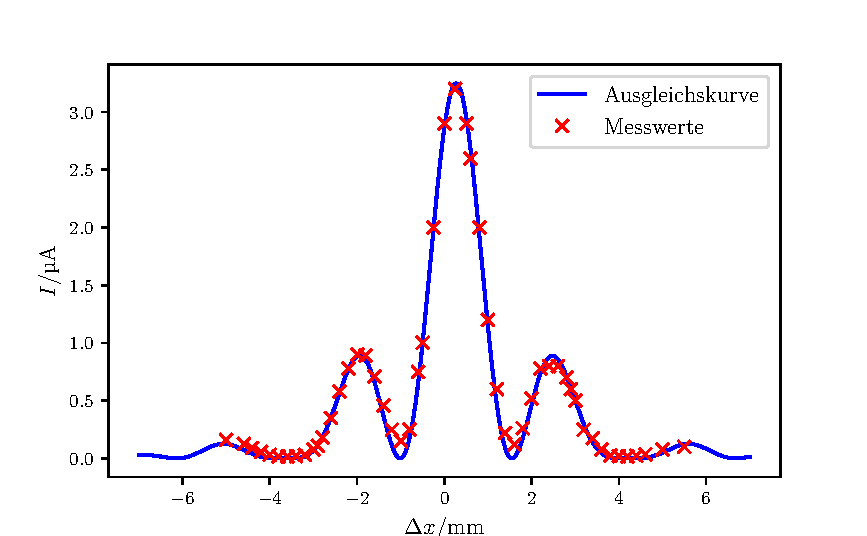
\includegraphics[width=\linewidth-70pt,height=\textheight-70pt,keepaspectratio]{content/images/Doppelspalt1.pdf}
\caption{Interferenzmuster der Stromintensitäten des 1.Doppelspalts in Abhängigkeit von der Verschiebung des Detektors}
\label{fig:Doppel1}
\end{figure}

\begin{figure}
\centering
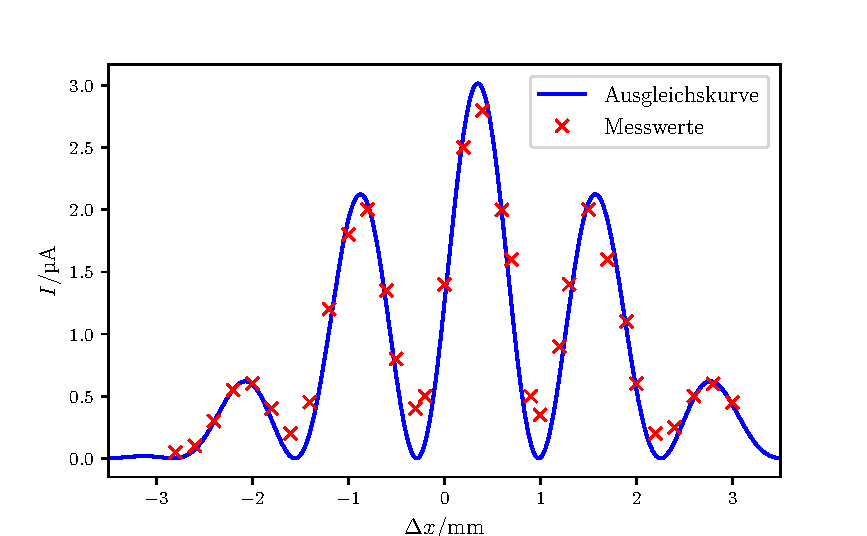
\includegraphics[width=\linewidth-70pt,height=\textheight-70pt,keepaspectratio]{content/images/Doppelspalt2.pdf}
\caption{Interferenzmuster der Stromintensitäten des 1. Doppelspalts in Abhängigkeit von der Verschiebung des Detektors}
\label{fig:Doppel2}
\end{figure}